\documentclass{article}

% if you need to pass options to natbib, use, e.g.:
% \PassOptionsToPackage{numbers, compress}{natbib}
% before loading nips_2016
%
% to avoid loading the natbib package, add option nonatbib:
% \usepackage[nonatbib]{nips_2016}

%\usepackage{nips_2016}

% to compile a camera-ready version, add the [final] option, e.g.:
\usepackage[final]{nips_2016}

\usepackage[utf8]{inputenc} % allow utf-8 input
\usepackage[T1]{fontenc}    % use 8-bit T1 fonts
\usepackage{hyperref}       % hyperlinks
\usepackage{url}            % simple URL typesetting
\usepackage{booktabs}       % professional-quality tables
\usepackage{amsfonts}       % blackboard math symbols
\usepackage{nicefrac}       % compact symbols for 1/2, etc.
\usepackage{microtype}      % microtypography




\usepackage[style=numeric,backend=bibtex,maxbibnames=99]{biblatex}
\addbibresource{references.bib}

\usepackage{graphicx}
\usepackage{caption}
\usepackage{subcaption}
\usepackage{float}
\usepackage{amsmath,amsfonts,amsthm,bm} % Math packages

\graphicspath{{img/}} %Setting the graphicspath




\title{Removing Noise from Speech with Deep Learning}

% The \author macro works with any number of authors. There are two
% commands used to separate the names and addresses of multiple
% authors: \And and \AND.
%
% Using \And between authors leaves it to LaTeX to determine where to
% break the lines. Using \AND forces a line break at that point. So,
% if LaTeX puts 3 of 4 authors names on the first line, and the last
% on the second line, try using \AND instead of \And before the third
% author name.

\author{
	Glávits Balázs \\
	Department of Measurement and Information Systems\\
	Budapest University of Technology and Economics\\
	\texttt{glavits.balazs@gmail.com} \\
	 \And
	Kiss Andor \\
	Department of Automation and Applied Informatics\\
	Budapest University of Technology and Economics\\
	\texttt{kissandor4@gmail.com} \\	 
	 \And
	Konrád Márk \\
	Department of Telecommunications and Media Informatics\\
	Budapest University of Technology and Economics\\
	\texttt{konrad0816@gmail.com} \\
	%% \AND
	%% Coauthor \\
	%% Affiliation \\
	%% Address \\
	%% \texttt{email} \\
	%% \And
	%% Coauthor \\
	%% Affiliation \\
	%% Address \\
	%% \texttt{email} \\
	%% \And
	%% Coauthor \\
	%% Affiliation \\
	%% Address \\
	%% \texttt{email} \\
}

\begin{document}
	% \nipsfinalcopy is no longer used
	
	\maketitle
	
	\begin{abstract}
		TODO
	\end{abstract}
	\newpage
	\section{Task summary}
	\label{sec:summary}
		Our goal is to reduce (or in the best case, entirely remove) the noise from audio recordings containing noisy speech. The idea is to use the WaveNet\cite{wavenet} architecture to generate clean audio from the noisy one.
		
	\section{Different approaches}
	In the research phase of our task we found several different implementations of speech denoising deep neural networks. The best ones are:
	\begin{itemize}
		\item \textbf{Speech Enhancement Generative Adversarial Network (SEGAN)}\cite{pascual2017segan}, which is a GAN based approach where the generator receives the noisy data with a latent representation and the discriminator is just a binary classifier.
		\item \textbf{Speech Enhancement based on Denoising Autoencoder with Multi-branched Encoders
		}\cite{yu2020speech}
		\item \textbf{WaveNet}\cite{wavenet}, which is a generative model aimed at creating raw audio waveforms. We experimented with several implementations. These can be seen in sections \ref{sec:wavenet} and \ref{sec:experiments}.
	\end{itemize}

	After considering these different solutions we decided to create an implementation based on the WaveNet architecture.
		
	\section{Data acquisition and exploration}
	For our training and testing data, we used a dataset called "\href{https://datashare.is.ed.ac.uk/handle/10283/2791}{Noisy speech database for training speech enhancement algorithms and TTS models}"\cite{dataset} by the University of Edinburgh. It consists of $\sim$23000 clean-noisy pairs (Figure \ref{fig:clean_noisy_noise}) from 56 different speakers. 
	The samples are stored in separate .wav files of varying length (Figure \ref{fig:dur}).  

	\begin{figure}[H]
		\centering
		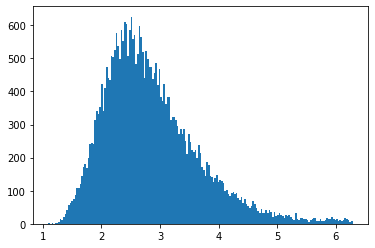
\includegraphics[width=.5\linewidth]{durations}
		\caption{Duration distribution histogram of a subset of speeches}
		\label{fig:dur}
	\end{figure}

	\begin{figure}[H]
		\centering
		\begin{subfigure}{.5\textwidth}
			\centering
			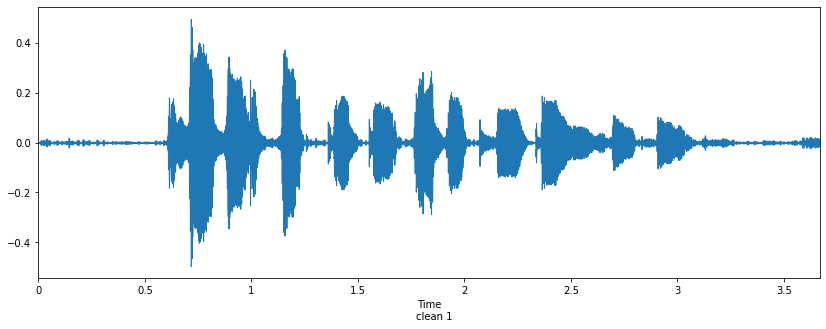
\includegraphics[width=.8\linewidth]{wave_for_noise_clean}
			\caption{clean}
			\label{fig:wave_for_noise_clean}
		\end{subfigure}%
		\begin{subfigure}{.5\textwidth}
			\centering
			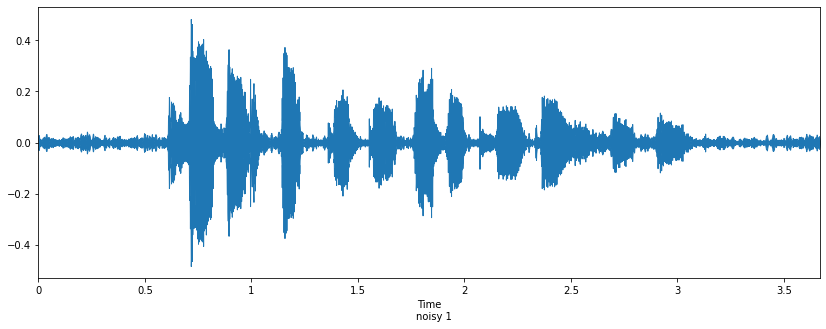
\includegraphics[width=.8\linewidth]{wave_for_noise_noisy}
			\caption{noisy}
			\label{fig:wave_for_noise_noisy}
		\end{subfigure}
		\label{fig:clean_noisy_n}
		
		\begin{subfigure}{.7\textwidth}
			\centering
			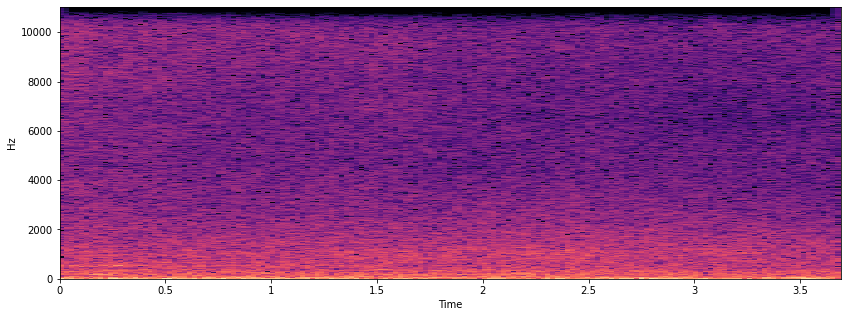
\includegraphics[width=.8\linewidth]{noise}
			\caption{noise spectogram}
			\label{fig:noise}
		\end{subfigure}
		\caption{Noisy and clean samples and the spectogram of the noise from the audio in figures \ref{fig:wave_for_noise_clean} and \ref{fig:wave_for_noise_noisy}}
		\label{fig:clean_noisy_noise}
	\end{figure}

	

	\section{Data preprocessing}

	Our first approach was to select the $n$ closest audio samples and zero-pad them to be the same duration, then reduce the samples to 8 bit with $\mu$-law transformation (figure \ref{fig:clean_noisy_padded_mulaw}).
	
	\begin{figure}[H]
		\centering
		\begin{subfigure}{.5\textwidth}
			\centering
			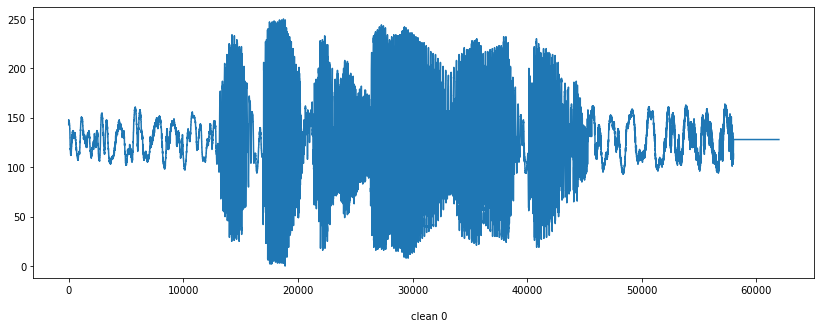
\includegraphics[width=.8\linewidth]{wave_clean_padded_mulaw}
			\caption{clean}
			\label{fig:wave_clean_padded_mulaw}
		\end{subfigure}%
		\begin{subfigure}{.5\textwidth}
			\centering
			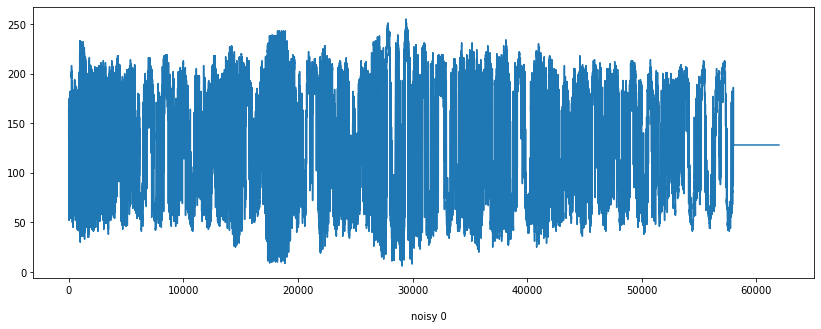
\includegraphics[width=.8\linewidth]{wave_noisy_padded_mulaw}
			\caption{noisy}
			\label{fig:wave_noisy_padded_mulaw}
		\end{subfigure}
		\caption{An example clean-noisy pair after padding and $\mu$-law transformation}
		\label{fig:clean_noisy_padded_mulaw}
	\end{figure}
	
	With this implementation we ran into the problem of limited hardware resources so, we had to come up with a less resource-intensive preprocessing pipeline.
	
	Our solution was to load the raw data, normalize it between -1 and 1 and downsample it to 16kHz. After these preprocessing steps, we feed the audio to the model with a data generator which can generate batches of smaller same sized pieces of data.
	With this approach, we eliminated the memory problem but sacrificed some of the continuity in our speech samples. The other upside of this solution is that we don't have to feed the meaningless data to the model in the form of zeroes.
	
	The original implementation of the WaveNet architecture used one-hot encoded $\mu$-law transformed data, but after experimenting with these, we could not generate audio with acceptable quality.


	\section{The WaveNet architecture}
	\label{sec:wavenet}
	For our network architecture, we choose to use a modified version of the WaveNet\cite{wavenet} architecture developed by DeepMind.

	WaveNet is a deep neural network capable of generating raw audio waveforms. This can be achieved with the use of a dilated causal convolutional layers. Causal means that the network is only conditioned on past and current inputs. With this approach, we can make sure that the ordering of the data is not violated. With dilation, we can achieve a large receptive field with the preservation of the input resolution. The structure of a stack created with these kinds of layers can be seen in Figure \ref{fig:dccs}.
	
		
	\begin{figure}[H]
		\centering
		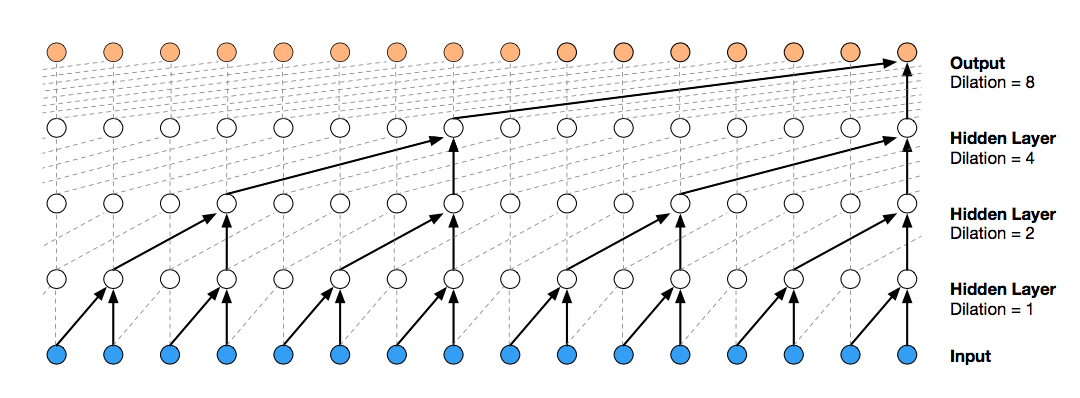
\includegraphics[width=.8\linewidth]{dccs.png}
		\caption{A dilated causal convolutional layer stack}
		\label{fig:dccs}
	\end{figure}
	
	The model uses residual blocks and skip connections to speed up the convergence and enable the use of deeper networks.
	
	\begin{figure}[H]
		\centering
		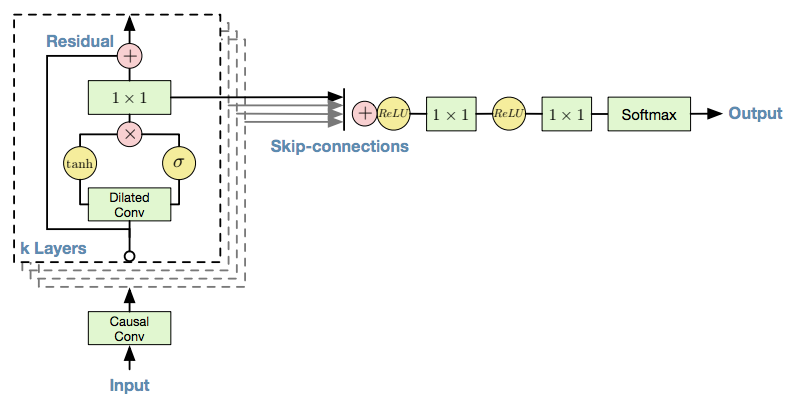
\includegraphics[width=.8\linewidth]{residual.png}
		\caption{Residual blocks in WaveNet}
		\label{fig:residual}
	\end{figure}

	To avoid making assumptions of the output shape the model uses discrete softmax distribution. The overview of the architecture can be seen in Figure \ref{fig:wavenet}.

	\begin{figure}[H]
		\centering
		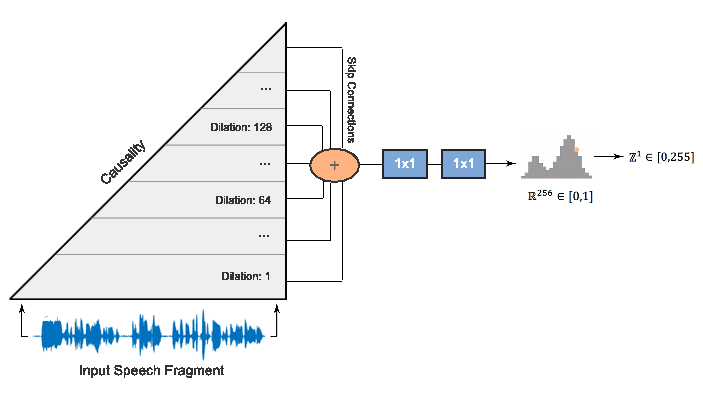
\includegraphics[width=.8\linewidth]{wavenet_overview.png}
		\caption{A simplified overview of the WaveNet architecture}
		\label{fig:wavenet}
	\end{figure}
	It must be noted that this model is primarily designed to be used in Text-to-Speech (TTS) applications.
	
	
	
	\subsection{WaveNet for noise removing}
	While the WaveNet architecture proposed by DeepMind is a state of the art implementation for TTS applications its current form is not suitable for speech denoising.
	Rethage et al. \cite{rethage2018wavenet} proposed a WaveNet adaptation for the purpose of removing noise from speech samples (Figure \ref{fig:wavenet2}).
	
	\begin{figure}[H]
		\centering
		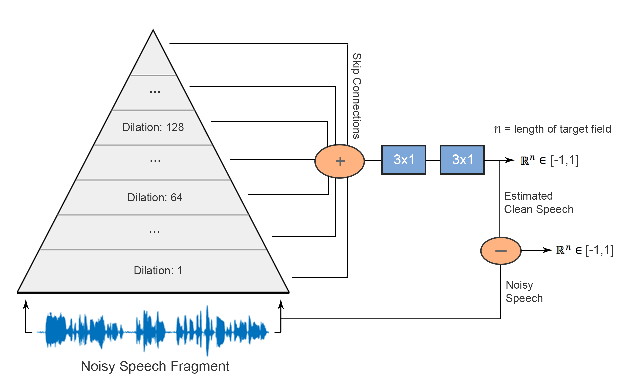
\includegraphics[width=.8\linewidth]{wavenet_overview2.png}
		\caption{A simplified overview of the WaveNet speech denoising architecture}
		\label{fig:wavenet2}
	\end{figure}
	
	The original WaveNet architecture uses causal convolutional layers for keeping the ordering of the data, but in speech denoising a substantially more accurate prediction can be achieved with non-causal convolutions. This change essentially doubled the context available to the model (Figure \ref{fig:dnccs}).
	
	
	\begin{figure}[H]
		\centering
		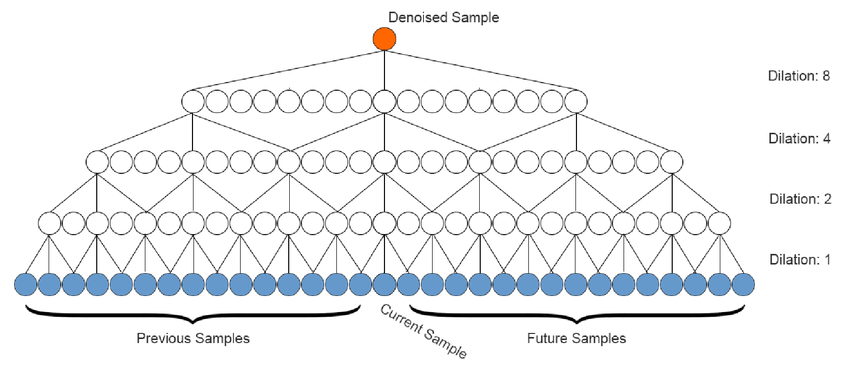
\includegraphics[width=.9\linewidth]{dnccs.png}
		\caption{A dilated non-causal convolutional layer stack}
		\label{fig:dnccs}
	\end{figure}
	
	
	\subsection{Our denoising WaveNet implementation}
	\label{sec:own_wavenet}
	To solve the problem proposed in section \ref{sec:summary}, we created our denoising WaveNet implementation. It consists of a stack of dilated non-causal convolutional layers with skip connections and three additional one-dimensional convolutional layers (Conv1D) to incorporate features extracted at every hierarchical level. The first two Conv1D layers have 2048 and 256 filters with the filter size of three and, the last one has one filter with the size of one. This structure can be seen in figure \ref{fig:own_wavenet}.
	\begin{figure}[H]
		\centering
		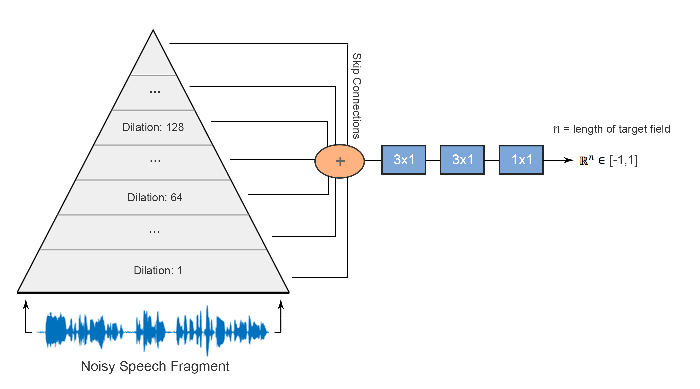
\includegraphics[width=.9\linewidth]{own_wavenet.png}
		\caption{Overview of the denoising WaveNet architecture}
		\label{fig:own_wavenet}
	\end{figure}
	
	
	
		\begin{figure}[H]
		\centering
		\begin{subfigure}{.5\textwidth}
			\centering
			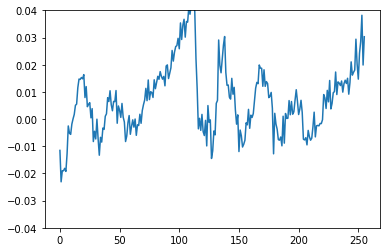
\includegraphics[width=.8\linewidth]{test_noisy}
			\caption{Noisy}
			\label{fig:test_noisy}
		\end{subfigure}%
		\begin{subfigure}{.5\textwidth}
			\centering
			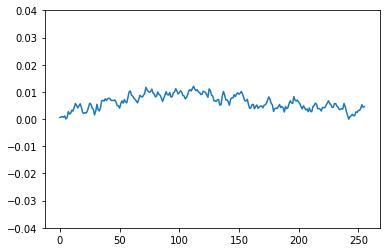
\includegraphics[width=.8\linewidth]{test_clean_orig}
			\caption{Clean}
			\label{fig:test_clean_orig}
		\end{subfigure}
		\begin{subfigure}{1\textwidth}
			\centering
			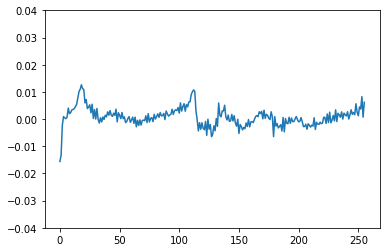
\includegraphics[width=.7\linewidth]{test_clean}
			\caption{Output}
			\label{fig:test_clean}
		\end{subfigure}
		\caption{An example noise reduction}
		\label{fig:test}
	\end{figure}
	
	
	\section{Experiments}
	\begin{itemize}
	\item \textbf{WaveNet with non-causal convolutions, \boldmath$\mu$-law transform and softmax distribution} \\
	At first, we tried to create a denoising model with dilated non-causal convolutional layers and, $\mu$-law transformed one-hot encoded input data. After some test runs, we decided to try another approach because, with this attempt, we could not reduce the noise on the samples at all.
	\item \textbf{WaveNet with non-causal convolutions, regression, and dense output layer} \\
	After the first failed experiment, we tried to skip the $\mu$-law transform step and move towards a regression-based model. In this attempt, we used dilated non-causal convolutions with a dense layer for output. The resulting quality was questionable because the network removed part of the clean speech along with some of the noise.
	\item \textbf{WaveNet with non-causal convolutions, regression, and flatten + dense output layers} \\
	This model was the first that could provide reasonably good output. The thought process behind the addition of a flatten layer was that with it there are be more connections in the network, and the output weights will be conditioned on the output of the convolutional layers and will eventually generate clean speech. It could remove most of the noise, but the quality of the speech was much worse than the input. The other downside of this model was that the training was extremely slow because of the size of the network.
	\item \textbf{WaveNet + auto-encoders} \\
	We tried to stack a denoising auto-encoder on top of a non-causal WaveNet because we thought that by giving the latent space from the WaveNet's output to an auto-encoder, we could decrease the noise even more. Unfortunately, this attempt could not even replicate the input speech.
	\item \textbf {Auto-encoder surrounded with WaveNets} \\
	Another attempt consisting of a combination of WaveNets and an auto-encoder was the idea of surrounding an auto-encoder with two identical WaveNets. We experienced a steady decrease in the model's loss, but unfortunately, we did not have the resources and time to test this model more.
	\item \textbf{WaveNet with non-causal convolutions, regression, and extra one dimensional convolutional layers on the output} \\
	Our final model is a WaveNet with non-causal convolutions followed by three one dimensional convolutional layers with filter sizes three, three, one. The output is promising because it can eliminate most of the noise and, the deterioration of the sound quality is much better than any of our past attempts. With more computation time on a machine with specialized resources, there is a chance that the sound quality will improve more. For more information about this model, refer to section \ref{sec:own_wavenet}.
	
	\end{itemize}



	
	
	\section{Future plans}
	\label{sec:experiments}
	
	\newpage
	\printbibliography



\end{document}